\documentclass[10pt,a4paper]{report}
\usepackage[utf8]{inputenc}
\usepackage[spanish]{babel}
\usepackage{amsmath}
\usepackage{amsfonts}
\usepackage{amssymb}
\usepackage{makeidx}
\usepackage{graphicx}
\usepackage{titlesec}
\usepackage{sectsty}
\usepackage{listings}
\usepackage{color}
\usepackage{float}
\usepackage{hyperref}
\usepackage{apacite}

\titleformat{\chapter}[display]
{\normalfont\bfseries}{}{0pt}{\Large}
\chaptertitlefont{\Huge}

\definecolor{codegreen}{rgb}{0,0.6,0}
\definecolor{codegray}{rgb}{0.5,0.5,0.5}
\definecolor{codepurple}{rgb}{0.58,0,0.82}
\definecolor{backcolour}{rgb}{0.95,0.95,0.92}

\lstdefinestyle{mystyle}{
	backgroundcolor=\color{backcolour},   
	commentstyle=\color{codegreen},
	keywordstyle=\color{magenta},
	numberstyle=\tiny\color{codegray},
	stringstyle=\color{codepurple},
	basicstyle=\footnotesize,
	breakatwhitespace=false,         
	breaklines=true,                 
	captionpos=b,                    
	keepspaces=true,                 
	numbers=left,                    
	numbersep=5pt,                  
	showspaces=false,                
	showstringspaces=false,
	showtabs=false,                  
	tabsize=2,
	frame=lines
}

\lstset{style=mystyle}

\author{David Alberto Medina Medina
	\\
	Dr. Modesto Fernando Castrillon Santana}
\title{Práctica 6 y 7 :\\ Procesamiento de imagen y video, \\y síntesis de sonido}
\begin{document}
	\maketitle
	\tableofcontents
	\bibliographystyle{apacite}
	\chapter{Introducción}
	\textit{Processing} es un es un IDE \textit{opensource} que utiliza \textit{Java} como lenguaje de programación. Este proyecto está desarrollado y mantenido por la \textit{Processing Foundation} que sirve como soporte de aprendizaje para instruir a estudiantes de todo el mundo en el mundo de la codificación dentro del contexto de las artes visuales.
	
	El objetivo de esta experiencia consite en desarrollar una aplicación de realidad aumentada desde la cual se puede interactuar con objetos virtuales en un espacio tridimensional y generar audio a partir de ellos. El modelo de una guitarra eléctrica es elegido en un intento de ilustrar esta funcionalidad. 
	
	En la escena se muestra la estructura de un esqueleto humano resultado de un algoritmo de seguimiento del cuerpo que procesa la \textit{Kinect v1.8} obteniendo como resultado la información de los puntos de articulación del mismo \cite{kinect-controller}. 
	
	La \textit{Kinect} solo ofrece la posición de cada punto de articulación en el plano XY por lo que es necesario analizar la información que de los sensores IR si queremos conocer la profundidad de cada uno de los puntos de articulación que conforman el esqueleto.
	
	\chapter{Método y materiales}
	\section{Materiales}
	El desarrollo de este proyecto se ha llevado a cabo utilizando el IDE de desarrollo de aplicaciones \textit{Java} de \textit{JetBrains}, \textit{IntelliJ}, y las siguientes herramientas:
	\begin{itemize}
		\item Librería \textit{Processing} \cite{processing-javadoc}.
		\item Librería \textit{Kinect4WinSDK} \cite{kinect4winsdk}.
		\item Librería \textit{Sound} \cite{sound-library}.
		\item Modelo \textit{OBJ} de una guitarra eléctrica \cite{3d-guitar-model}.
	\end{itemize}
	
	\section{Método}
	Las siguientes clases que se definenen en este documente se organizan en los siguientes paquetes:
	\begin{enumerate}
		\item main
		\item kinect
		\item soundFX
		\item object
		\item algorithms
	\end{enumerate}

	\subsection{Paquete \texttt{main}}
	\subsubsection{Clase \texttt{KinectMe}}\label{class:kinectme}
	Para poder utilizar las primitivas de \textit{Processing} esta clase debe heredar de \texttt{PApplet}. Para iniciar una aplicación de \textit{Processing}, el método estático \texttt{main()} debe llamar a la primitiva \texttt{PApplet.main()} para indicar el nombre de la clase principal desde la cual se llama y sobrescriben los métodos primitivos: \texttt{settings(), setup()} y \texttt{draw()}.
	
	\lstinputlisting[language=Java, firstline=162, lastline=164]{../src/main/KinectMe.java}
	
	El método primitivo \texttt{settings()} establece el tamaño de la pantalla llamando al método \texttt{size()} y pasándole la marca del renderizador de gráficos 3D (\texttt{P3D}).
	
	\lstinputlisting[language=Java, firstline=24, lastline=28]{../src/main/KinectMe.java}
	
	El método \texttt{setup()} inicializa un objeto de la clase \texttt{Kinect} --además, de establecer el radio de acción de las manos-- que se utiliza como controlador de la misma. Además, se llama al método \texttt{spawnGuitar()} responsable del renderizado y puesta en escena de una guitarra que será el objeto tridimensional por medio del cual el usuario puede interactuar. El método \texttt{createFloor()} permite visualizar una rejilla que será utilizada como suelo de la escena.
	
	\lstinputlisting[language=Java, firstline=30, lastline=42]{../src/main/KinectMe.java}
	
	El método privado \texttt{spawnGuitar()} carga el modelo 3D de la guitarra y le asigna una posición en la escena. El método \texttt{doDrawInteractionArea()} permite visualizar los volúmenes de interacción asociados a la guitarra si ajustamos el parámetro \texttt{DEBUG\_AREAS} a \texttt{true}.
	
	A continuación, se llama al método privado \texttt{addGuitarInteraction()} para generar los ortoedros de interacción a partir de los cuales el usuario puede interacturar con la guitarra. Se generan dos volúmenes de interacción: uno para el cuello y el otro para las cuerdas de la guitarra. Es posible visualizar los vértices de estos ortoedros si se establece el parámetro de configuración \texttt{DEBUG\_VERTICES} a \texttt{true}.
	
	\lstinputlisting[language=Java, firstline=44, lastline=81]{../src/main/KinectMe.java}
	
	El método \textit{createFloor()} genera una malla que representará el suelo del mundo.
	
	\lstinputlisting[language=Java, firstline=120, lastline=133]{../src/main/KinectMe.java}
	
	El método primitivo \texttt{draw()} refresca los elementos de la escena y son mostrados por pantalla para su visualización. Se habilita al controlador de la \textit{Kinect} mostrar el esqueleto por pantalla y el suelo del mundo. 
	
	\lstinputlisting[language=Java, firstline=84, lastline=97]{../src/main/KinectMe.java}	
	
	La posición de la cámara en función de la posición del punto de articulación de la columna del esqueleto detectado por la \textit{Kinect} al llamar al método \texttt{setCamera()}.
	
	\lstinputlisting[language=Java, firstline=99, lastline=111]{../src/main/KinectMe.java}
	
	El estado de la guitarra --resultado de la interacción del usuario con los volúmenes de interacción defnidos para la misma-- se actualiza con cada llamada al método \texttt{guitarInteraction()}, así como su posición en el mundo.
	
	 \lstinputlisting[language=Java, firstline=135, lastline=148]{../src/main/KinectMe.java}
	 
	 El suelo se muestra por pantalla al llamar al método \texttt{makeFloor()}.
	 
	 \lstinputlisting[language=Java, firstline=113, lastline=118]{../src/main/KinectMe.java}
	 
	 Cada vez que aparezca, desaparezca o se mueva algún punto de articulación por la pantalla se procede a llamar a los eventos correspondientes.
	 
	 \lstinputlisting[language=Java, firstline=150, lastline=160]{../src/main/KinectMe.java}
	
	
	\subsection{Paquete \texttt{kinect}}
	\subsubsection{Clase \texttt{Kinect}}\label{class:kinect}
	Esta clase es la interfaz que permite interactuar con la \textit{Kinect v1.8}. El constructor acepta los siguientes parámetros:
	\begin{description}
	\item[parent] Es una referencia a un objeto de la clase principal \texttt{KinectMe}.
	\item[pos] Establece al posición inicial en el espacio tridimensional de la imágenes obtenidas desde la \textit{Kinect v1.8}.
	\item[scale] Establece la escala de la imagen.
	\item[skeletonRGB] Se trata de un vector que ajusta el color del esqueleto que se muestra por pantalla.
	\end{description}
	
	\lstinputlisting[language=Java, firstline=30, lastline=44]{../src/kinect/Kinect.java}
	
	El método \texttt{refresh()} permite refrescar las imágenes que se muestran por pantalla así como visualizar el esqueleto detectado por la \textit{Kinect}. El primer parámetro de este método es un selector de la clase \texttt{KinectSelector} permite elegir entre las diferentes opciones de visualización. El segundo parámetro, es una variable booleana que permite visualizar por pantalla las imágenes obtenidas de la \textit{Kinect} cuando se asigna a \texttt{true}.
	
	\lstinputlisting[language=Java, firstline=75, lastline=117]{../src/kinect/Kinect.java}
	
	El método \texttt{bodyTracking()} muestra por pantalla todos los esqueletos detectados por la \textit{Kinect} con cada llamada al método \texttt{drawSkeleton()}. Este último, sondea todos los puntos de articulación que conforman el esqueleto detectado e imprime por pantalla cada una de las partes que conforman el esqueleto.
	
	\lstinputlisting[language=Java, firstline=119, lastline=144]{../src/kinect/Kinect.java}
	
	Los puntos son sondeados con la llamada al método \texttt{collectPoints()}.
	
	\lstinputlisting[language=Java, firstline=164, lastline=170]{../src/kinect/Kinect.java}
	
	Cada una de las partes que componen el esqueleto son construidas llamando al método correspondiente. Cada método realiza una llamada a \texttt{DrawBone()} con dos selectores de puntos de articulación (\texttt{KinectAnathomy}) como argumentos.
	
	\lstinputlisting[language=Java, firstline=172, lastline=229]{../src/kinect/Kinect.java}
	
	\texttt{DrawBone()} toma dos selectores de articulación y pinta una línea entre esos dos puntos originando, de este modo, una articulación. 
	
	En el caso de pintar el punto de articulación de las manos, se comprueba si el radio es mayor que 0. Si es así, se pinta una esfera del radio que se ha especificado. 
	
	\lstinputlisting[language=Java, firstline=231, lastline=262]{../src/kinect/Kinect.java}
	
	La gestión de los eventos mencionados al final de la sección \ref{class:kinectme} son llevado a cabo por los métodos \texttt{appearEvent(), disappearEvent()} y \texttt{moveEvent()}.
	
	\lstinputlisting[language=Java, firstline=264, lastline=295]{../src/kinect/Kinect.java}
	
	
	\subsubsection{Enumerado \texttt{KinectAnathomy}}
	Este enumerado identifica los diferentes puntos de articulación detectados por la \textit{Kinect v1.8}.
	
	\lstinputlisting[language=Java, firstline=14, lastline=51]{../src/kinect/KinectAnathomy.java}
	
	Las coordenadas de cada punto de articulación --incluida la profundidad-- son calculadas en el método \texttt{getJointPos()}.
	
	\lstinputlisting[language=Java, firstline=53, lastline=61]{../src/kinect/KinectAnathomy.java}
	
	El cálculo de la profundidad se obtiene a partir de la imagen en blanco y negro que devuelve la librería \texttt{Kinect4WinSDK} tras llamar a la primitiva \texttt{GetDepth()}.
	
	Para establecer la profundidad de cada punto de articulación se analiza cada uno de los píxeles de la imagen devuelta por \texttt{GetDepth()} y se toma el byte menos significativo. Posteriormente, se comprueba que el valor del byte se encuentre en el rango umbral del intervalo $\left[ 100, 250\right]$. El rango de profundidad se establece en el intervalo $\left[ 0, 360\right]$ y se asigna este valor al punto de articulación correspondiente.
	
	\lstinputlisting[language=Java, firstline=63, lastline=85]{../src/kinect/KinectAnathomy.java}
	
	
	\subsubsection{Enumerado \texttt{KinectSelector}}
	Este enumerado permite seleccionar entre el tipo de imagen que se desea mostrar por pantalla:
	\begin{itemize}
	\item RGB
	\item DEPTH
	\item MASK
	\item NONE
	\end{itemize}
	
	\lstinputlisting[language=Java, firstline=3, lastline=8]{../src/kinect/KinectSelector.java}
	
	
	\subsection{Paquete \texttt{object}}
	\subsubsection{Clase \texttt{Object}}
	Esta clase abstracta contiene un constructor que toma como parámetros de entrada el modelo del objeto (\texttt{PShape}), las texturas (\texttt{Texture}) y el material (\texttt{Material}).
	
	\lstinputlisting[language=Java, firstline=7, lastline=28]{../src/object/Object.java}
	
	Se puede acceder a estas propiedades a través de sus \texttt{getters}.
	
	\lstinputlisting[language=Java, firstline=53, lastline=75]{../src/object/Object.java}
	
	La posición y ángulos de rotación de un objeto presentan también sus propios \textit{getters} y \textit{setters}. Cada vez que se actualiza la posición o el ángulo de rotación del objeto, se modifican también los parámetros de posición y rotación de los volumenes de interacción asociados al mismo.
	
	\lstinputlisting[language=Java, firstline=29, lastline=51]{../src/object/Object.java}
	
	El objeto puede ser escalado llamando al método \texttt{scale()}.
	
	\lstinputlisting[language=Java, firstline=85, lastline=87]{../src/object/Object.java}
	
	Cada objeto dispone de una lista de objetos \texttt{InteractiveVolume} que designa los volúmenes de interacción con los que podrá interactuar el usuario. Esta lista dispone a su vez del siguiente \textit{getter} y \textit{setter}.
	
	\lstinputlisting[language=Java, firstline=77, lastline=83]{../src/object/Object.java}
	
	Se puede actualizar el estado de un objeto \texttt{SceneObject} llamando al método \texttt{refresh()}. El material, textura y posición de una instancia de esta clase son actualizados con cada iteración de \texttt{draw()}. Las traslaciones y rotaciones que se lleven a cabo en el objeto son aplicadas llamando al método \texttt{setTransformations()}. El estado del objeto es actualizado llamando al método \texttt{updateState()}.
	
	\lstinputlisting[language=Java, firstline=89, lastline=106]{../src/object/Object.java}
	
	Otros métodos abstractos que se declaran en esta clase son:
	\begin{description}
		\item[\texttt{updateState()}.] Actualizar el estado de los volúmenes de interacción asociados al objeto.
		\item[\texttt{touched()}.] Lanza las respuestas necesarias cuando un volumen de interacción es tocado por un usuario.
		\item[doDrawInteractionVolume().] Permite dibujar los volúmenes de interacción cuando se asigna su parámetro a \texttt{true}.
		\end{description}	
	
	 \lstinputlisting[language=Java, firstline=106, lastline=110]{../src/object/Object.java}
	
	\subsubsection{Clase \texttt{Texture}}
	Esta clase es la responsable de almacenar las texturas de una instancia del objeto \texttt{SceneObject}.
	
	\lstinputlisting[language=Java, firstline=6, lastline=18]{../src/object/Texture.java}
	
	\subsubsection{Clase \texttt{Material}}
	Esta clase es la responsable de gestionar los parámetros de los materiales que son utilizados por los objetos de la escena. Estos parámetros controlan cómo se comporta cada objeto de la escena ante la luz. El método \texttt{refresh()} es el responsable de llamar a las primitivas en cada iteración.
	
	\lstinputlisting[language=Java, firstline=14, lastline=63]{../src/object/Material.java}
	
	\subsubsection{Clase \texttt{InteractionVolume}}
	Los volúmenes de interacción asociados a un objeto son definidos en esta clase. Su constructor toma los siguientes argumentos:
	\begin{description}
	\item[parent.] Es una referencia a un objeto de la clase principal \texttt{KinectMe}.
	\item[id.] Una \textit{string} que identifica el tipo de volumen de interacción que se va a generar.
	\item[width.] Número de tipo \texttt{float} que asigna el ancho del volumen de interacción.
	\item[height.] Número de tipo \texttt{float} que asigna el alto del volumen de interacción.
	\item[depth.] Número de tipo \texttt{float} que asigna la profundidad del volumen de interacción.
	\end{description}
	
	\lstinputlisting[language=Java, firstline=31, lastline=49]{../src/object/InteractiveVolume.java}
	
	El campo \texttt{id} tiene su propio \textit{getter}.
	
	\lstinputlisting[language=Java, firstline=51, lastline=53]{../src/object/InteractiveVolume.java}
	
	La posición y ángulo de rotación del volumen interactivo tienen definidos sus propios \textit{getters} y \textit{setters}. Los \textit{setters} añaden siempre el espaciado necesario para ubicar el volumen en la posición que le corresponde en el objeto.
	
	\lstinputlisting[language=Java, firstline=55, lastline=73]{../src/object/InteractiveVolume.java}
	
	El punto de contacto del usuario con el volumen de interacción dispone de sus propios \textit{getter} y \textit{setter}.
	
	\lstinputlisting[language=Java, firstline=75, lastline=81]{../src/object/InteractiveVolume.java}
	
	Los métodos \texttt{isTouchedLeft()} e \texttt{isTouchedRight()} indican si un volumen de interacción ha sido tocado con la mano izquierda o derecha, respectivamente.
	
	\lstinputlisting[language=Java, firstline=83, lastline=89]{../src/object/InteractiveVolume.java}
	
	El centroide de un volumen de interacción se obtiene a partir del método \texttt{getCentroid()}.
	
	\lstinputlisting[language=Java, firstline=145, lastline=161]{../src/object/InteractiveVolume.java}
	
	El volumen de interacción es generado gracias al método \texttt{generateBoxVolume()}.
	
	\lstinputlisting[language=Java, firstline=91, lastline=129]{../src/object/InteractiveVolume.java}
	
	El método \texttt{isColliding()} identifica si un punto de articulación del esqueleto a tocado o colisionado con el volumen de interacción. La colisión es detectada siguiendo el algoritmo de colisiones de cajas delimitadores \cite{3d-collision-detection}.
	
	\lstinputlisting[language=Java, firstline=163, lastline=206]{../src/object/InteractiveVolume.java}
	
	Si efectivamente se ha colisionado con el volumen de interacción el método privado \texttt{isTouched()} indica qué mano lo ha tocado y se ajusta el color de relleno del volumen a verde. Si no ha habido ninguna colisión el color del volumen se asigna a un color rojo.
	
	\lstinputlisting[language=Java, firstline=208, lastline=224]{../src/object/InteractiveVolume.java}
	
	Si se desea visualizar los vértices y el centroide del volumen de interacción y el punto de articulación de las manos se llama al método privado \texttt{visualizeVertexAndHand}.
	
	\lstinputlisting[language=Java, firstline=226, lastline=232]{../src/object/InteractiveVolume.java}
	
	Las traslaciones y rotaciones del volumen de interacción poseen sus propios \textit{getters} y \textit{setters}.
	
	\lstinputlisting[language=Java, firstline=238, lastline=252]{../src/object/InteractiveVolume.java}
	
	El método \texttt{refresh()} coloca el volumen de interacción en el espacio asignando las rotaciones y traslaciones pertinentes.
	
	\lstinputlisting[language=Java, firstline=131, lastline=143]{../src/object/InteractiveVolume.java}
	
	\subsubsection{Clase \texttt{Guitar}}
	Se trata de una subclase de \texttt{Object} que sobrescribe los métodos \texttt{toched()} y \texttt{updateStates()}. Esta clase se ubica dentro del paquete \texttt{object.intrument}.
	
	El método \texttt{touched()} detecta por cada volumen de interacción asociado a la guitarra --el cuello y las cuerdas de la guitarra-- si ha habido alguna colisión de las manos izquierda o derecha. 
	
	Si ha ocurrido una colisión con la caja de interacción del cuello de la guitarra, se asigna a las coordenadas del punto de contacto del volumen de interacción las del punto de articulación de la mano que colisionó con él. 
	
	Si la colisión ocurre en la caja de interacción de las cuerdas de la guitarra entonces se llama al método \texttt{play()} de la clase \texttt{SoundFX} para reproducir un sonido generado por un oscilador a elección.
	
	Si por el contrario, no ha habido ninguna colisión de las manos con los volúmenes del cuello de la guitarra, entonces se moverá la guitarra en bloque junto con sus volúmenes de interacción asociados a la coordenada que indique la mano con la que colisionó.
	
	En el caso de que se deje de interactuar con el volumen de las cuerdas, se detendrá la reproducción del sonido generado por la guitarra.
	
	\lstinputlisting[language=Java, firstline=26, lastline=66]{../src/object/InteractiveVolume.java}
	
	El método privado que permite mover la guitarra en bloque hacia el punto de articulación de la mano cuando se deja de tocar el cuello de la guitarra es \texttt{moveToJoint()}.
	
	\lstinputlisting[language=Java, firstline=68, lastline=72]{../src/object/InteractiveVolume.java}
	
	El método público \texttt{updateState()} permite actualizar la posición y rotación de los volúmenes de interacción asociados a la guitarra.
	
	\lstinputlisting[language=Java, firstline=74, lastline=82]{../src/object/InteractiveVolume.java}
	
	\subsection{Paquete \texttt{sounFX}}
	\subsubsection{Clase \texttt{SoundFX}}
	Esta clase define el generador de audio asociado a la guitarra eléctrica usando diferentes osciladores.
	
	Si se quiere generar un sonido, se debe pasar al método \texttt{play()} el selector de oscilador que se desea utilizar para reproducir el sonido así como un número \texttt{float} que inidique la frecuencia del mismo. Cada vez que se llama a este método se asigna a 0 el valor de \texttt{sustain} que permite que la nota se siga sonando después de un cierto tiempo tras llamar al método \texttt{stop()}.
	
	\lstinputlisting[language=Java, firstline=39, lastline=68]{../src/soundFX/SoundFX.java}
	
	El método \texttt{stop()} permite detener el sonido una vez campo \texttt{sustain} haya alcanzado el umbral definido por \texttt{SUSTAIN\_TIME}.
	
	\lstinputlisting[language=Java, firstline=70, lastline=95]{../src/soundFX/SoundFX.java}
	
	\subsubsection{Enumerado \texttt{OscillatorSelector}}
	Este enumerado permite seleccionar entre los diferentes tipos de osciladores disponibles por la librería \texttt{Sound} para generar sonido.
	
	\lstinputlisting[language=Java, firstline=3, lastline=9]{../src/soundFX/SoundFX.java}
	
	\chapter{Resultados y Discusión}
	El algoritmo integrado de seguimiento de cuerpo que dispone la \texttt{Kinect v1.8} ha permitido establecer una nube de puntos de referencia a partir de los cuales ha sido posible seguir la posición en 2D de los puntos de articulación del cuerpo. 
	
	Ha sido posible establecer un correlación de los valores de profundidad de cada punto de articulación a partir de la imagen en blanco y negro generado por la primitiva \texttt{GetDepth()} de la librería \texttt{Kinect4WinSDK} generados a partir de los sensores IR de la \textit{Kinect v1.8}.
	
	El resultado final es un prototipo de realidad aumentada que permite interaccionar con un objeto para moverlo por un espacio virtual y generar sonido a partir de él. 
	
	Su utilidad podría expandirse para generar una nube de puntos en un espacio tridimensional gracias a sus sensores IR y generar un modelo 3D a partir de ellos.
		
	\begin{figure}[h]
		\centering
		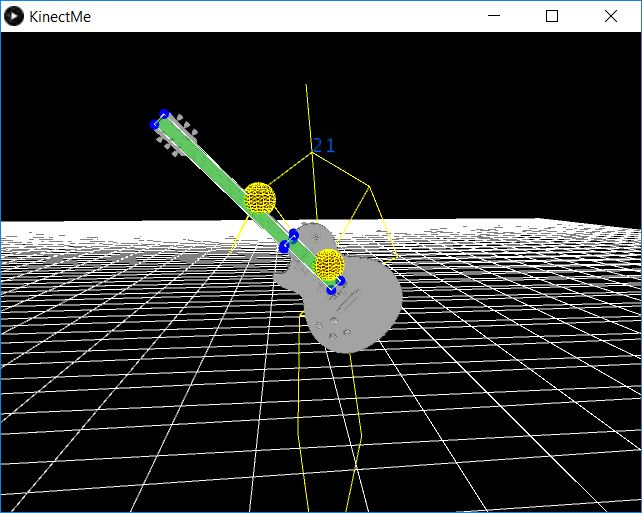
\includegraphics[width=0.9\textwidth]{KinectMe.png}
		\caption{Espacio virtual desde el que se puede interaccionar utilizando el algoritmo de detección de cuerpos de la \textit{Kinect}}
	\end{figure}
	
	\chapter{Conclusiones}	
	La \textit{Kinect} es una herramienta muy útil para realizar el seguimiento de objetos es un espacio tridimensional así como la estimación de profundidad de cualquier cuerpo que se encuentre dentro del rango de acción de los sensores IR.
	
	Estas características convierten a la \textit{Kinect} en un dispositivo económico para realizar funciones de seguimiento del movimiento o definición de nubes de puntos de cualquier cuerpo tridimensional en industrias como la animación.
	
	\bibliography{Report-6-7}
\end{document}